\chapter{Einführung}
Secure Multiparty Computation ist ein großes Forschungsfeld in der Kryptographie. In diesem Bereich begann die Forschung zwar schon in den 1980er Jahren, unter anderem mit Arbeiten von Yao \cite{Yao1982}, seit den 2000er Jahren bekommt die Secure Computation jedoch deutlich mehr Aufmerksamkeit. Das ist unter anderem im Anstieg der Anzahl der Veröffentlichungen pro Jahr in diesem Bereich zu sehen \cite{Kogan2021}. 
In diesem Forschungsfeld werden Methoden erforscht, mit denen gemeinsam Funktionen von Eingabedaten berechnet werden können, ohne dass dabei die anderen teilnehmenden Parteien die Eingabedaten erhalten.\\
Die Forschungen in den 80er Jahren haben die theoretischen Grundlagen der Forschung geliefert und sich beispielsweise damit beschäftigt, welche Berechnungen überhaupt möglich sind. Die Forschung in den letzten Jahren ist jedoch eher praktisch, das Ziel ist es also die Fortschritte auch in Anwendungen nutzbar zu machen \cite{Kogan2021}.\\
Durch mehrere Effekte wurden die Berechnungen erst in breiteren Anwendungsbereichen sinnvoll nutzbar. Einerseits wurden die berechnenden Computer stärker, beispielsweise hat sich unter Anderem die CPU Geschwindigkeit in PCs ungefähr verdoppelt. Das allein kann aber noch nicht die mehr als 60.000 fache Beschleunigung der Berechnungsgeschwindigkeit \cite{Kogan2021} erklären. 
\begin{figure}[H]
\begin{center}
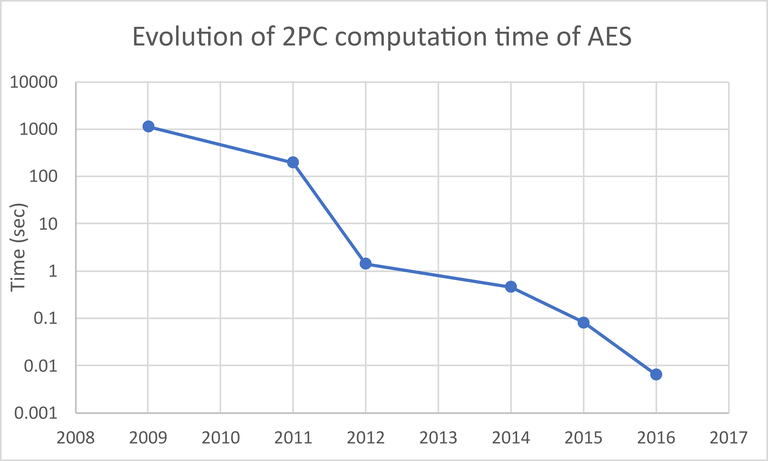
\includegraphics[width = 8cm]{comptime.png}
\caption{
Die Grafik \ref{evolution_of_computation} stellt dar\, wie sich die Geschwindigkeit der Secure Computation über die Jahre verändert hat.
Auf der Y-Achse die Berechnungszeit in Sekunden in einer logarithmischen Skala angegeben. Abgebildet ist, wie lange das zu diesem Zeitpunkt schnellste Secure Computation Protokoll für die Berechnung von AES bei der Beteiligung von zwei Parteien benötigt.\\
}
\cite{Kogan2021}
\label{evolution_of_computation}
\end{center}

\end{figure}

Durch die Grafik \ref{evolution_of_computation} wird die sich immer weiter verbessernde Geschwindigkeit der Secure Computation Protokolle deutlich. Zur leichteren Lesbarkeit und besseren Vergleichbarkeit zeigt die Grafik zwar nur die Berechnungszeiten für zwei Parteien, dennoch wird deutlich, dass sich durch die Forschung in diesem Bereich die Effizienz von Secure Computation Protokollen stark gesteigert hat. Der größte Teil des Tempogewinns liegt also an den neu entwickelten oder verbesserten Protokollen.\\
Eine Funktion, die in vielen Bereichen interessant sein kann, ist die Schnittmenge der Eingabemengen der teilnehmenden Parteien, auch PSI für \glqq Private Set Intersection\grqq{} genannt. 2021 veröffentlichten Branco et al. \cite{Doettling2021} ein Paper, in dem ein neues Protokoll vorgestellt wurde, das die threshold-Variante dieser Funktion erfüllt. Durch eine Effizienzanalyse kann man nun feststellen, wie schnell dieses Protokoll in der Praxis sein kann.

\section{Anwendungsbeispiel}
Die Entwickler des Tor Browser, den Menschen benutzen können, um in das sogenannte Darknet zu gelangen, legen einen sehr großen Wert auf die Sicherheit der Nutzer. Das macht die Analyse bestimmter Statistiken sehr schwierig. Deshalb gibt es auch vom Anbieter selbst keine genauen Angaben über beispielsweise die Nutzerzahl, sondern nur Schätzungen. Um genauere Schätzungen über die Nutzerzahl zu ermöglichen, könnte man nun Daten von mehreren \glqq Knoten\grqq{} des Tor Netzwerks kombinieren. In diesem Fall möchte man gerne herausfinden, wie viele Überschneidungen es in den Daten der \glqq Knoten\grqq{} gibt, um Mehrfachzählungen zu vermeiden. Da viele Nutzer des Tor Browsers aber einen sehr großen Wert auf Sicherheit legen, möchte man natürlich vermeiden, Daten von mehreren \glqq Knoten\grqq{} miteinander zu kombinieren, weil so möglicherweise Informationen gewonnen werden könnten, die geheim bleiben sollten.\\
Um zu garantieren, dass die Daten beispielsweise nur zur Ermittlung der Größe der Schnittmenge genutzt werden, können spezielle Protokolle genutzt werden, die die Daten nur verschlüsselt benutzen und nur ganz bestimmte  Analysen der verschlüsselten Daten erlauben. So kann man Statistiken über das Netzwerk des Tor Browsers erstellen, ohne dass die Gefahr besteht, dass Informationen der Nutzer zugänglich werden.

\section{Zielsetzung}
Das Ziel der Arbeit ist es, die praktische Effizienz und Geschwindigkeit der im Paper von Branco et al. \cite{Doettling2021} vorgestellten neuen Teilprotokolle zu testen. \\
Um alle Teilprotokolle wie im Paper beschrieben zu implementieren, sind auch Implementierungen von anderen Veröffentlichungen nötig (\cite{Schoenmakers} Beispielsweise für das secureRank Teilprotokoll). Da zu diesem Zeitpunkt noch keine derartigen Implementierungen veröffentlicht sind, kann ich auch nicht auf diese zurückgreifen. Um die Teilprotokolle, die im Paper von Branco et al. \cite{Doettling2021} beschrieben sind, trotzdem analysieren zu können, habe ich die Unterprotokolle, die auf solche externen Paper zurückgreifen auf unsichere Weise implementiert. Das heißt, dass in meiner Implementierung dieser Teilprotokolle auch der Secret Key der Verschlüsselung benutzt wird, um Informationen zu entschlüsseln. Danach kann man dann übliche Algorithmen nutzen, um das korrekte Ergebnis der Berechnung zu erhalten, das dann wieder verschlüsselt wird.\\
Diese anderen Veröffentlichungen ebenfalls selbst zu implementieren würde über den Rahmen dieser Arbeit hinaus gehen. Für die genutzten Funktionen der Paper gibt es jedoch Schätzungen, die es ermöglichen, die Berechnungsdauer vorherzusagen.\\
Durch diese Nachbildung der Funktionalität kann das Protokoll getestet werden und die Tests können zumindest genaue Daten für die Berechnungen in den korrekt implementierten Protokollen geben.
